\documentclass[a4paper]{article}


\usepackage[margin=2cm]{geometry}
\usepackage{tikz}
\usepackage{float}
\usepackage[english]{babel}
\usepackage{csquotes}
\usepackage{amsmath, amssymb, amsfonts}
\usepackage{mathtools}
\usepackage{subcaption}


\usepackage{hyperref}

\usetikzlibrary{positioning, arrows, automata}

\tikzset{
  % state/.style={
  %   draw, circle
  % },
  -latex,auto,node distance=1cm, semithick
}

\setlength{\parindent}{0cm}

\begin{document}

\title{Networking}
\author{Joan Marcè i Igual}

\maketitle

% !TEX root = ../main.tex

\section{Model behaviour using labelled transistion system (LTS)}

We have multiple interfaces with

An automaton for a simple light:
\begin{itemize}
  \item Input:
  \begin{itemize}
    \item Switch on
    \item Switch off
  \end{itemize}
  \item Output:
  \begin{itemize}
    \item Light on
    \item Light off
  \end{itemize}
\end{itemize}

There are two states:
\begin{itemize}
  \item On
  \item Off
\end{itemize}

The inputs switch from one state to the other, label transition system, 
\autoref{fig:deterministic_on}

\begin{figure}
  \centering
  \begin{subfigure}[b]{.45\textwidth}
    \centering
    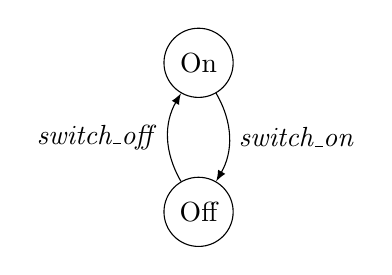
\begin{tikzpicture}
      \tikzstyle{every state}=[draw]

      \node[state] (on) {On};
      \node[state, below = of on] (off) {Off};

      \path (on)    edge[bend left] node {\emph{switch\_on}}  (off)
            (off)   edge[bend left] node {\emph{switch\_off}} (on);
      
    \end{tikzpicture}

    \caption{Simple automata \label{fig:deterministic_on}}
  \end{subfigure}
  ~
  \begin{subfigure}[b]{.45\textwidth}
    \centering
    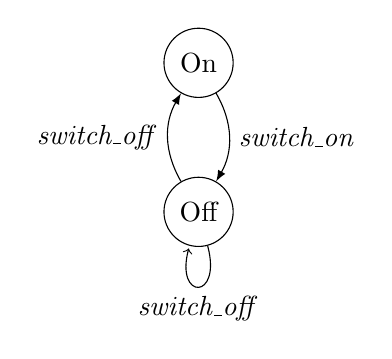
\begin{tikzpicture}
      \tikzstyle{every state}=[draw]
      
      \node[state] (on) {On};
      \node[state, below = of on] (off) {Off};
      
      \path (on)    edge[bend left]   node {\emph{switch\_on}}  (off)
      (off)   edge[bend left]   node {\emph{switch\_off}} (on)
      edge[loop below]  node {\emph{switch\_off}} (off);
      
    \end{tikzpicture}
    
    \caption{Non-deterministic automata \label{fig:non-deterministic_on}}
  \end{subfigure}
\end{figure}
Sometimes we have a non-deterministic behaviour \autoref{fig:non-deterministic_on}. We can go
to two different states coming from the same previous state and having the same input

\subsection{Definition of a labelled transition system}

Definition
\textbf{This is a test}


\subsection{Transition system with an infinite state space}

Example: the natural numbers

\begin{align*}
  S &= \{ 0, 1, 2, 3, ... \} \\
  Act &= \{ Up, Down \}  \\
  \rightarrow &= \{ <i, Up, i+1>, <i, Down, i-1> \}
\end{align*}

If we were to remove the transition from 2 and 3 we would have unreachable states



% !TEX root = ../main.tex

\section{Behavioural equivalences}

\subsection{When transition systems are equal?}

\begin{figure}[H]
  \centering
  \begin{subfigure}[b]{.4\textwidth}
    \centering
    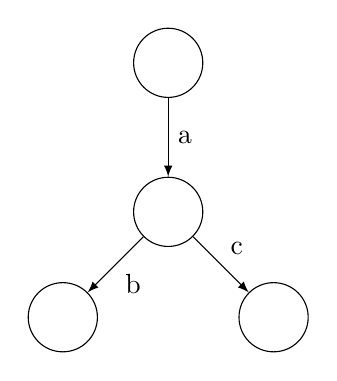
\begin{tikzpicture}
      \node[state] (0) {};
      \node[state, below = of 0] (1) {};
      \node[state, below left = of 1] (2) {};
      \node[state, below right = of 1] (3) {};

      \draw (0)   edge    node {a}  (1)
            (1)   edge    node {b}  (2)
                  edge    node {c}  (3);
    \end{tikzpicture}
    \caption{System a \label{fig:02_system_a}}
  \end{subfigure}
  ~
  \begin{subfigure}[b]{.4\textwidth}
    \centering
    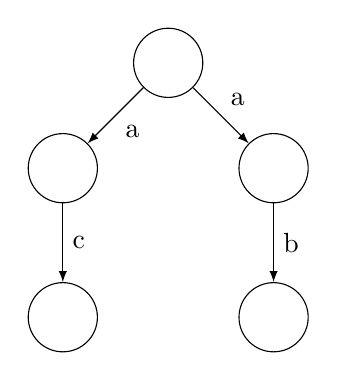
\begin{tikzpicture}
      \node[state] (0) {};
      \node[state, below right = of 0] (1) {};
      \node[state, below left = of 0] (2) {};
      \node[state, below = of 1] (3) {};
      \node[state, below = of 2] (4) {};

      \draw (0)   edge    node {a}  (1)
                  edge    node {a}  (2)
            (1)   edge    node {b}  (3)
            (2)   edge    node {c}  (4);
    \end{tikzpicture}
    \caption{System a \label{fig:02_system_b}}
  \end{subfigure}
  \caption{Are these two systems equivalent?}
\end{figure}



Usually it depends in the interaction on when two systems are equal. 
Not \emph{bisimulation equivalent}.


\subsection{Bisimulation equivalence}

We say that a relation \( \pmb{R} \subseteq S \times S \) is a bisimulation relation iff for all states
\( s,t \in S \) it holds that if \( sRt \).

\begin{itemize}
  \item if \( s \xrightarrow{a} s' \) for some \( s'\in S\), then there is some \( t' \in S \)
  such that \( t \xrightarrow{a} t' \) and \( s'\pmb{R}t' \).
  \item if \( t \xrightarrow{a} t' \) for some \( t'\in S\), then there is some \( s' \in S \)
  such that \( s \xrightarrow{a} t' \) and \( s'\pmb{R}t' \).
  \item \( s \in T \) iff \( t \in T \)
\end{itemize}

Two states \( s,t \in S \) are called bisimilar 


\textbf{Theorem} Every transition system has a \emph{unique} minimal transition system that is
bisimulation equivalent to it.

\begin{figure}[H]
  \centering
  \begin{subfigure}[b]{.45\textwidth}
    \centering
    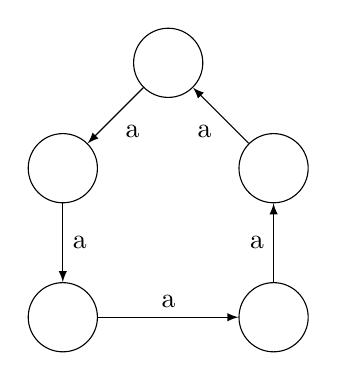
\begin{tikzpicture}
      \node[state] (0) {};
      \node[state, below left = of 0] (1) {};
      \node[state, below right = of 0] (2) {};
      \node[state, below = of 1] (3) {};
      \node[state, below = of 2] (4) {};

      \draw (0)   edge    node {a}    (1)
            (1)   edge    node {a}    (3)
            (3)   edge    node {a}    (4)
            (4)   edge    node {a}    (2)
            (2)   edge    node {a}    (0);
    \end{tikzpicture}
    \caption{System a}
  \end{subfigure}
  \centering
  \begin{subfigure}[b]{.45\textwidth}
    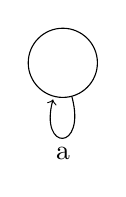
\begin{tikzpicture}
      \node[state] (0) {};
      
      \draw (0) edge[loop below] node {a} (0);
    \end{tikzpicture}
    \caption{System b}
  \end{subfigure}
  \caption{These two systems have a bisimulation relation}
\end{figure}

\subsection{Trace equivalence}


\begin{figure}[H]
  \begin{subfigure}[b]{.4\textwidth}
    \centering
    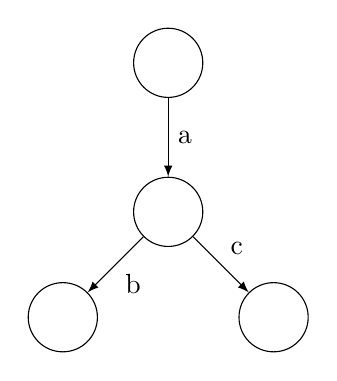
\begin{tikzpicture}
      \node[state] (0) {};
      \node[state, below = of 0] (1) {};
      \node[state, below left = of 1] (2) {};
      \node[state, below right = of 1] (3) {};

      \draw (0)   edge    node {a}  (1)
            (1)   edge    node {b}  (2)
                  edge    node {c}  (3);
    \end{tikzpicture}
    \caption{System a, trace is \( \{ \epsilon, a, a \cdot b, a \cdot c \} \)}
  \end{subfigure}
  ~
  \begin{subfigure}[b]{.4\textwidth}
    \centering
    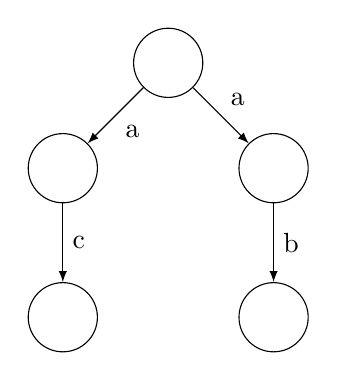
\begin{tikzpicture}
      \node[state] (0) {};
      \node[state, below right = of 0] (1) {};
      \node[state, below left = of 0] (2) {};
      \node[state, below = of 1] (3) {};
      \node[state, below = of 2] (4) {};

      \draw (0)   edge    node {a}  (1)
                  edge    node {a}  (2)
            (1)   edge    node {b}  (3)
            (2)   edge    node {c}  (4);
    \end{tikzpicture}
    \caption{System b, trace is \( \{ \epsilon, a, a \cdot b, a \cdot c \} \)}
  \end{subfigure}

  \caption{These two systems are not bisimilar but have a trace equivalence}
\end{figure}

For the trace equivalence all the partial traces are included. Trace equivalence does not 
preserve deadlocks. To verify a system, never use trace equivalence because it does not counts 
the deadlocks.

Calculating bisimulation on a finite transition system with \( n \) states and \( m \) transitions
requires \emph{insert formula here}

\begin{displayquote}
For deterministic transition systems bisimulation and trace equivalence coincide
\end{displayquote}

\subsection{Useful facts}

If you show that two transitions systems are not trace equivalent you could find one trace in 
one but not in the other.

Exercise from 20: Are these two trace equivalent? 

Yes these two are trace equivalent because we always have 3a followed by another letter. 

Exercise from 21: Are these two bisimilar?

No, they are not bisimilar because you can end in a transition where a b transition must be mimicked
by another b transition but this is not possible.


\subsection{Branching bisimulation}

A relation \(\pmb{R}\) is a \emph{branching bisimulation} relation iff, some branches can be 
skipped 

\begin{figure}[H]
  \centering
  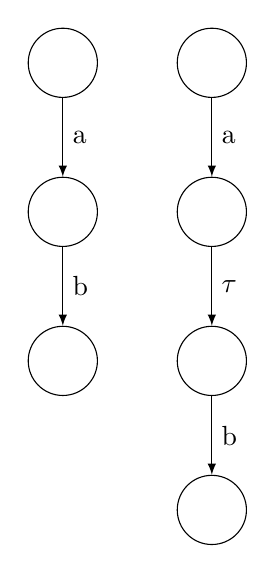
\begin{tikzpicture}
    \node[state] (a0) {};
    \node[state, below = of a0] (a1) {};
    \node[state, below = of a1] (a2) {};
    \node[state, right = of a0] (b0) {};
    \node[state, below = of b0] (b1) {};
    \node[state, below = of b1] (b2) {};
    \node[state, below = of b2] (b3) {};

    \draw (a0)    edge    node {a}    (a1)
          (a1)    edge    node {b}    (a2)
          (b0)    edge    node {a}    (b1)
          (b1)    edge    node {\(\tau\)}    (b2)
          (b2)    edge    node {b}    (b3);
  \end{tikzpicture}

  \caption{These two systems are branching bisimilar}
\end{figure}

\subsection{Combining behaviour}

If we combine branching bisimilar systems we do not obtain branching bisimilar systems.

\subsection{Rooted branching bisimulation}

A rooted branching bisimulation relation \( \pmb{R}\) is a branching bisimulation that also
satisfies that the first transition is the same, without skips.

Strong bisimulation implies rooted branching bisimulation implies branching bisimulation.

\subsection{When to use which behavioural equivalence?}

\begin{itemize}
  \item Strong bisimulation, always safe
  \item Trace equivalence, 
  \item Divergence preserving branching bisimulation. Used to remove internal steps. Always safe choice.
  \item Branching bisimulation. Safe choice when eventualities are not important, as it removes
  \(\tau\)-loops.
  \item Weak bisimulation. For practical purposes generally equivalent to branching bisimulation.
  \item Weak trace equivalence. Removes all \(\tau\)s. Does not preserve branching behaviour.
  Use with care.
\end{itemize}

Exercice I (pag. 43): We have a complex system where we hide many actions. We want to see whether
the behaviour is free from deadlocks. What should we use?

1) Strong bisimulation. It is always safe but we hide many actions, although correct it is not 
the best scenario
2) Divergence preserve branching bisimulation. Is is always safe, seems like the best choice
3) Branching bisimulation. In this case it is the safe choice, any deadlock that exists is going
to be preserved after branching bisimulation reduction.
4) Trace equivalence. No, it does not preserve deadlocks
5) It does not preserve deadlocks neither.

\subsection{Summary}

We defined the following behavioural equivalences:
\begin{itemize}
  \item (Weak) trace equivalence
  \item Strong bisimulation
  \item (Rooted) (Divergence preserving) branching bisimulation
\end{itemize}

We saw some guidelines on when to use which behavioural equivalence




% !TEX root = ../main.tex

\section{Specifying LTSs and applying behavioural equivalences}

\textbf{LTS}: Label Transition Systems

How can we actually use some of the tools for the project?


\textbf{Exercise}: Given the label transition system

\begin{figure}[H]
  \centering
  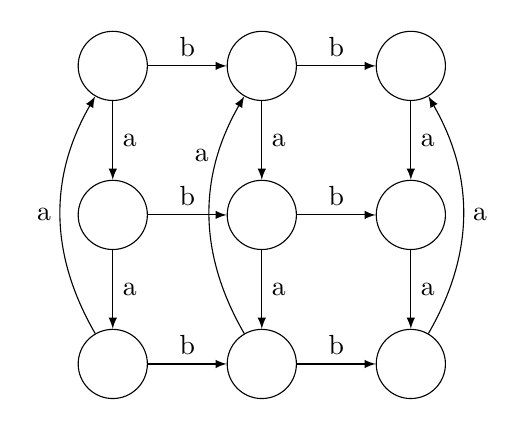
\begin{tikzpicture}
    \node[state] (aa) {};
    \node[state, below = of aa] (ba) {};
    \node[state, below = of ba] (ca) {};
    \node[state, right = of aa] (ab) {};
    \node[state, below = of ab] (bb) {};
    \node[state, below = of bb] (cb) {};
    \node[state, right = of ab] (ac) {};
    \node[state, below = of ac] (bc) {};
    \node[state, below = of bc] (cc) {};

    \draw
      (aa)    edge node[above] {b}    (ab)
              edge node[right] {a}    (ba)
      (ba)    edge node[above] {b}    (bb)
              edge node[right] {a}    (ca)
      (ca)    edge node[above] {b}    (cb)
              edge[bend left] node[left] {a} (aa)
      (ab)    edge node[above] {b}    (ac)
              edge node[right] {a}    (bb)
      (bb)    edge node[above] {b}    (bc)
              edge node[right] {a}    (cb)
      (cb)    edge node[above] {b}    (cc)
              edge[bend left] node[left, near end] {a} (ab)
      (ac)    edge node[right] {a}    (bc)
      (bc)    edge node[right] {a}    (cc)
      (cc)    edge[bend right] node[right] {a} (ac);
  \end{tikzpicture}
\end{figure}

\textbf{Exercise}: Slide 4, are these LTSs branching bisimilar?

We can relate the $\tau$ transition by doing nothing int the left LTS

\subsection{Goals}
\begin{itemize}
  \item Model small LTSs in mCRL2
  \item Explain what specification means
  \item Generate LTS from specification
  \item Apply behavioural equivalences to small examples
\end{itemize}

\subsection{Structure of the mCRL2 toolset}
The input is written as process algebra, something similar to a programming language to 
describe processes. Then it's linearized and linear process algebra is created, similar to an
assembly language. Finally a LTS is generated.

When specifying a system in mCRL2 the starting point are the actions. An action is, in fact, a 
LTS.

\subsubsection{Multi-actions}

Actions happening simultaneously

\begin{align*}
  & a | b \\
  & a | b | c \\
  & a | a \\
  & a | a | a |a  \\
  & \tau
\end{align*}

\subsubsection{Exercise II}

Are the following pairs of processes strongly bisimilar?

\begin{itemize}
  \item $a \cdot (b + c)$ and $a \cdot b + a \cdot c$. 

  No, these are not strongly bisimilar
  \item $a \cdot b + a \cdot b$ and $a \cdot b$
  \item $a \cdot b + a \cdot c$ and $(a + a) \cdot (b + c)$

  No, this is the same as the first case

\end{itemize}

\subsection{Transition systems with data}

Actions:
\begin{itemize}
  \item \emph{get(d)}
  \item \emph{deliver(d)}
\end{itemize}

$$
D = \{d_1, d_2\}
$$

\subsubsection{Alternating bit protocol}

When you have an unreliable transfer channel (e.g. internet)

You can get:
\begin{itemize}
  \item A successful transmission
  \item An unsuccessful transmission
\end{itemize}

You send a bit and expect an acknowledgement bit.

\subsection{Summary}
\begin{itemize}
  \item Modeled LTSs in mCRL2
  \item We generate LTSs from a specification
  \item We applied behavioural equivalences
  \item We saw how we can use tools and techniques to analyses a real protocol
  \item Tools used: mcrl2-gui, mcrl2ide, mcrl2xi, mcrl22lps, lps2lts, ltsconvert, ltscompare
\end{itemize}



% !TEX root = ../main.tex

\section{Abstract data types}

To model a model we need to be able to model the data too. Similar to functional programming.

\subsection{Goal}
\begin{itemize}
  \item Describe abstract data types (ADTs)
  \item Be able to use ADTs in mCRL2
\end{itemize}

\subsection{Declaration of data type}

\textbf{sort} D;

It represents a non-empty domain. $D$ can have infinite elements.

The most basic data type are the booleans.

\textbf{sort} $\mathbb{B}$;

\textbf{cons} \emph{true}, \emph{false}: $\mathbb{B}$

Special semantic rule: The elements representing \emph{true} and \emph{false} of sort $\mathbb{B}$
(\emph{Bool}) must be different.

\begin{align*}
  \text{\textbf{sort} } & \mathbb{B}; \\
  \text{\textbf{cons} } & true, false: \mathbb{B}; \\
  \text{\textbf{map} } & not: \mathbb{B} \Rightarrow \mathbb{B}; \\
  & and, or: \mathbb{B} \times \mathbb{B} \Rightarrow \mathbb{B}; \\
  \text{\textbf{var} } & b: \mathbb{B} \\
  \text{\textbf{eqn} } & not(true) = false; \\
  & not(false) = true; \\
  & not(not(true)) = true; \\
  \text{\textbf{eqn} } & and(true, b) = b; \\
  & and(false, b) = false; \\
  & and(b, true) = b; \\
  & and(b, false) = false; \\
  \text{\textbf{eqn}} & or(true, b) = true; \\
  & or(false, b) = b; \\
  & or(b, true) = true; \\
  & or(b, false) = b; \\
\end{align*}

\subsubsection{Induction/case distinction on Bool}
Can we prove $and(b, b) = b$ ?

As true and false are the constructors of $\mathbb{B}$ we only have to prove that 
$and(true, true) = true$ and that $and(false, false) = false$.

Prove that $and(b, c) = and(c, b)$:

\begin{align*}
  \text{case } & b = true \\
  & and(true, c) = c \\
  & \text{case } c = true \\
  & & and(true, true) = and(true, true) \\
  & \text{case } c = false \\
  & & \underbrace{and(true, false)}_{false} = \underbrace{and(false, true)}_{false} \\
\end{align*}

\subsection{Specification numbers. Peano arithmetic}

\begin{align*}
  \text{\textbf{sort} } & Nat; \\
  \text{\textbf{cons} } & zero: Nat; \\
  & succ: Nat \rightarrow Nat; \\
  \text{\textbf{map }} & add: Nat \times Nat \rightarrow; \\
  \text{\textbf{var }} & n, m: Nat; \\
  \text{\textbf{eqn }} & add(zero, zero) = zero; \\
  & add(zero, succ(n)) = succ(n); \\
  & add(succ(n), zero) = succ(n); \\
  & add(succ(n), succ(m)) = succ(add(n, succ(m))); \\
  \text{\textbf{map }} & <: Nat \times Nat \rightarrow \mathbb{B}; \\
  \text{\textbf{eqn }} & n < zero = false; \\
  & zero < succ(n) = true; \\
  & succ(n) < succ(m) = n < m;
\end{align*}

\begin{align*}
  & zero & 0 \\
  & succ(zero) & 1 \\
  & succ(succ(zero)) & 2 \\
\end{align*}

\subsubsection{Induction on Natural numbers}
Prove a property of \emph{zero}

Prove a property for $succ(n)$, assuming that it has been proven for $n$.

Then the property has been prover for all natural numbers $n$.

\subsection{Specification of efficient natural numbers}

Peano arithmetic is too inefficient for system validation.

\begin{align*}
  \text{sort } & \mathbb{N}^+; \qquad \text{sort } Pos;
\end{align*}

No maximum number

\subsection{Natural numbers}

\begin{align*}
  \text{sort } & \mathbb{N}; \qquad \text{sort} Nat; \\
  \text{cons } & @c0: \mathbb{N}; \\
  & @cNat: \mathbb{N}^+ \rightarrow \mathbb{N}; \\
  \text{map } & \simeq: \mathbb{N} \times \mathbb{N} \rightarrow \mathbb{N}^+
\end{align*}










\end{document}